
\section{Le Dipendenze }


La lezione inizia con la riproduzione di un video, patrocinato dal
Ministero della Salute, con la partecipazione di Nino Frassica, che ha
come scopo la promozione della salute e che riguarda determinati
atteggiamenti, quali ad esempio il fumo o l'utilizzo del casco. Per
produrre una campagna comunicativa come questa la prima cosa da fare è
identificare una popolazione target, poi i contenuti, che devono essere
scientificamente solidi, e infine un linguaggio adatto per raggiungere
quel determinato target. Spesso vengono utilizzati personaggi famosi per
fare maggiore presa sul pubblico.

La Dottoressa Odone mostra altri due video, frutto di un progetto di
collaborazione tra la Società Italiana Igiene e la Scuola del cinema di
Roma e Milano per la promozione delle vaccinazioni. In questi spot si
possono notare cenni di concetti scientifici spiegati al pubblico meno
esperto, come la ``herd immunity'' o le vaccinazioni dedicate agli
anziani.


\subsection{La dipendenza da sostanze}


La World Drug Report stima che 12 milioni di persone (la popolazione
mondiale è circa 7 miliardi) facciano uso di droghe iniettive, di cui
1,2 milioni sono HIV+ e 6 milioni hanno l'epatite C.

Per droga si intende una sostanza in grado di modificare il modo in cui
funzionano gli organi fisici e la mente. Esistono due tipi di
dipendenza:

\begin{itemize}
\item
  psichica
\item
  fisica, mediata da meccanismi biologici ben conosciuti.
\end{itemize}

È la combinazione delle due che rende la dipendenza una problematica di
sanità pubblica e una patologia classificata nel DSM come psichiatrica.
Possiamo definire droga una sostanza naturale o sintetica che si mette
in relazione con l'organismo umano, in grado di incidere sullo stato di
coscienza, alterando la percezione e incidendo sulle prestazioni
psicofisiche. Il concetto di dipendenza è un concetto di patologia, ma
l'utilizzo di droghe ha un forte impatto anche sul sistema
socio-sanitario con conseguenze dirette e indirette: cliniche sulla
persona singola che fa uso di droghe, che variano anche a seconda del
tipo di sostanza, ma anche sulla popolazione perché spesso il fenomeno
si associa ad aumento del tasso di criminalità, aumento della diffusione
di certe malattie, aumento degli incidenti/infortuni e soprattutto
aumento dei costi per il sistema sanitario, dovuto a certi servizi
offerti, come ad esempio quello del SERT.

Secondo il Ministero della Salute in Italia i consumatori di sostanze
stupefacenti nel 2011 (occasionali e abituali) sono circa 2,5 milioni.

Le classificazioni dei vari tipi di droghe (naturali e sintetiche) del
ministero sono dinamiche e vengono continuamente aggiornate man mano che
si censiscono nuove droghe.

\begin{figure}[!ht]
\centering
	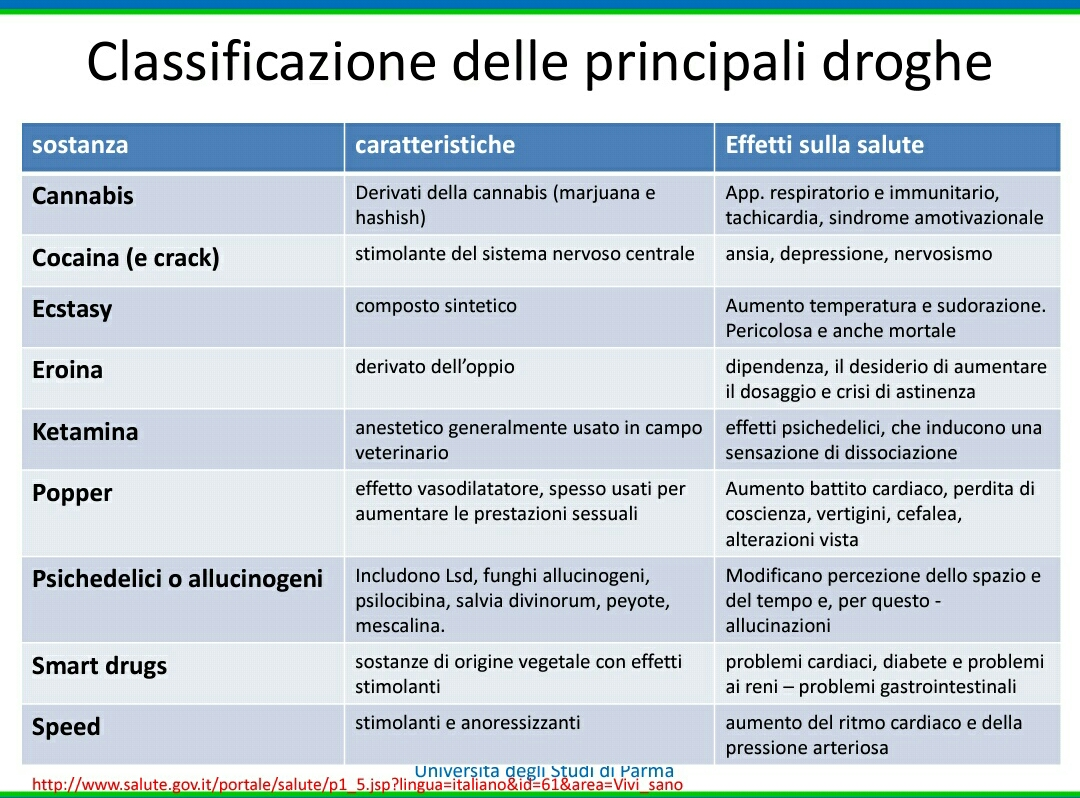
\includegraphics[width=0.7\textwidth]{18/image1.jpeg}
\end{figure}

Esistono agenzie europee, che sono organi di supporto su varie
tematiche. Ad esempio a Parma, c'è l'EFSA (agenzia europea per la
sicurezza alimentare) mentre a Lisbona c'è quella per il monitoraggio
delle dipendenze da droghe. Il suo ruolo è quello di fornire all'Unione
Europea e agli stati membri supporto tecnico per le decisioni prese a
livello comunitario in tema di politiche sanitarie, offrendo ai
policy-makers i dati e le informazioni che servono per fare
raccomandazioni e leggi, ma anche quello di aiutare i professionisti a
identificare quelle che sono le base-practices da implementare in quello
specifico campo d'azione. In particolare, questa agenzia di Lisbona
raccoglie dati sul consumo e li divulga.

Attualmente il trend consumo di droga in Europa è quello della
``poliassunzione'', ossia un approccio dipendente verso diversi tipi di
sostanze. In Europa si stima siano 88 milioni i giovani adulti
consumatori, circa un quarto della popolazione europea, con una quota
maggiore tra la popolazione maschile (55 milioni).

La sostanza più utilizzata è la \textbf{cannabis}: tra gli adulti, 19
milioni di persone dichiarano di averla assunta nell'ultimo anno,
equivalenti al 5,7\% della popolazione, mentre 79 milioni (23\%)
dichiarano di averla assunta nel corso della vita. Se invece si analizza
la fascia più a rischio, ovvero 15-34 anni, la percentuale di
consumatori nell'ultimo anno sale a 11\%.

\begin{figure}[!ht]
\centering
	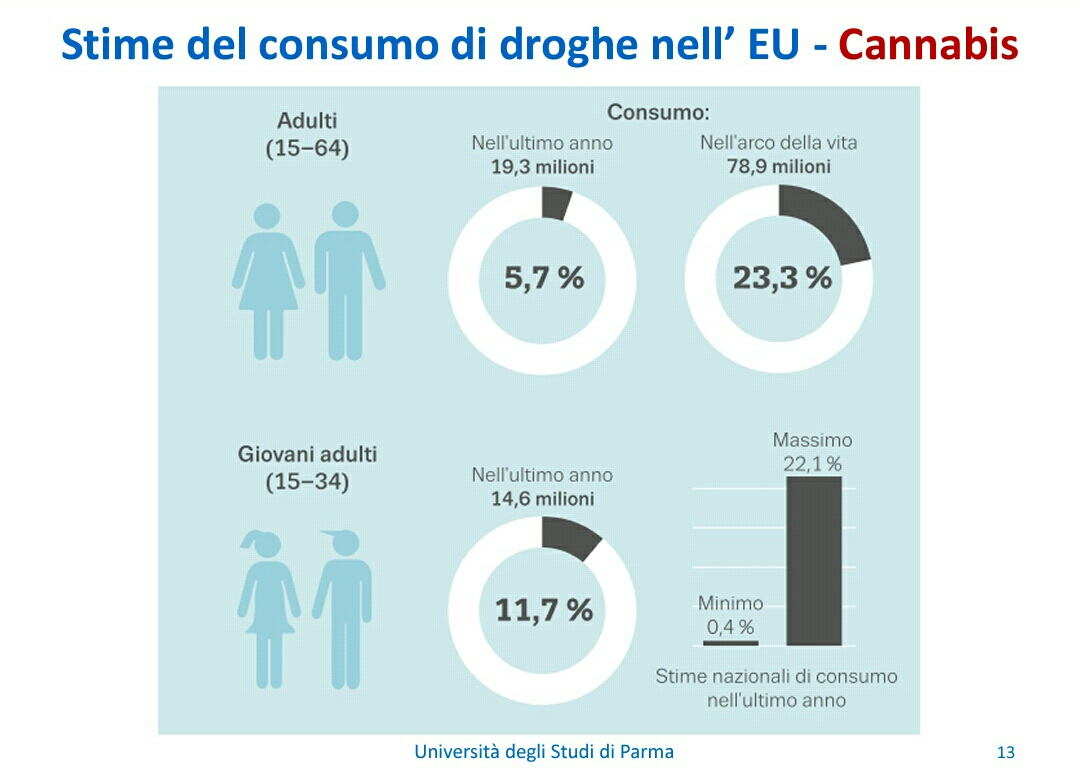
\includegraphics[width=0.7\textwidth]{18/image2.jpeg}
\end{figure}

Per quanto riguarda la \textbf{cocaina}, il 4,6\% della popolazione ne
ha fatto uso nell'arco della vita e l'1\% nell'ultimo anno. In questo
caso il gap tra adulti e giovani adulti è minore perché tra i più
giovani la percentuale è solo di poco superiore (1,9\%) a differenza di
quello che accade con la cannabis. Ovviamente questi dati si riferiscono
all'utilizzo e non alla dipendenza, quindi andrebbero analizzati poi i
modelli di assunzione perché un'assunzione saltuaria durante il weekend
è diversa da un'assunzione patologica da manuale.

\begin{figure}[!ht]
\centering
	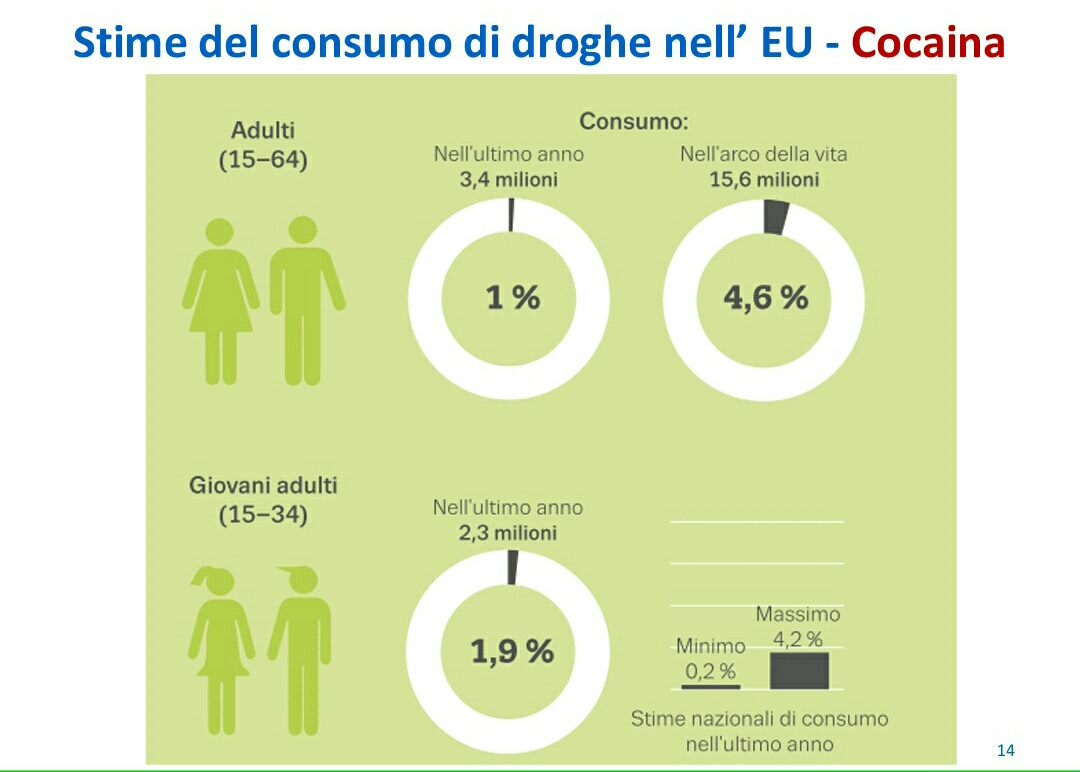
\includegraphics[width=0.7\textwidth]{18/image3.jpeg}
\end{figure}

\begin{figure}[!ht]
\centering
	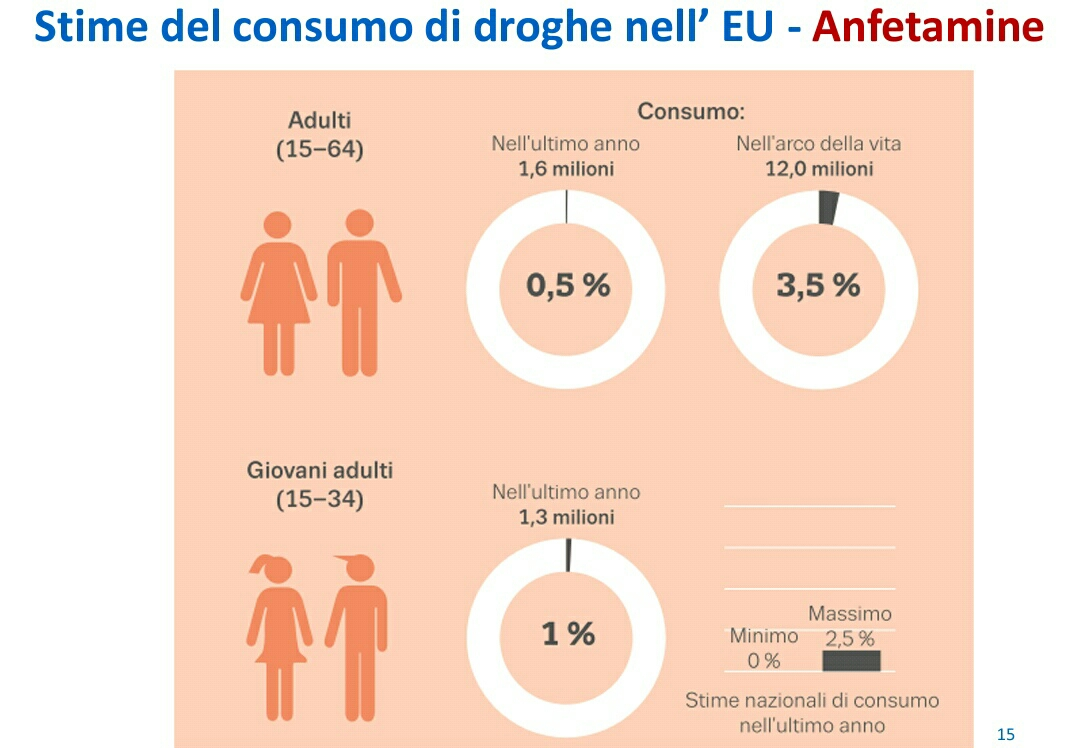
\includegraphics[width=0.7\textwidth]{18/image4.jpeg}
\end{figure}

Le \textbf{anfetamine} vengono
consumate dal 3,5\% della popolazione nell'arco della vita, mentre per
quanto riguarda il consumo nell'ultimo anno si stima lo 0,5\% tra gli
adulti e l'1\% tra i più giovani.

\begin{figure}[!ht]
\centering
	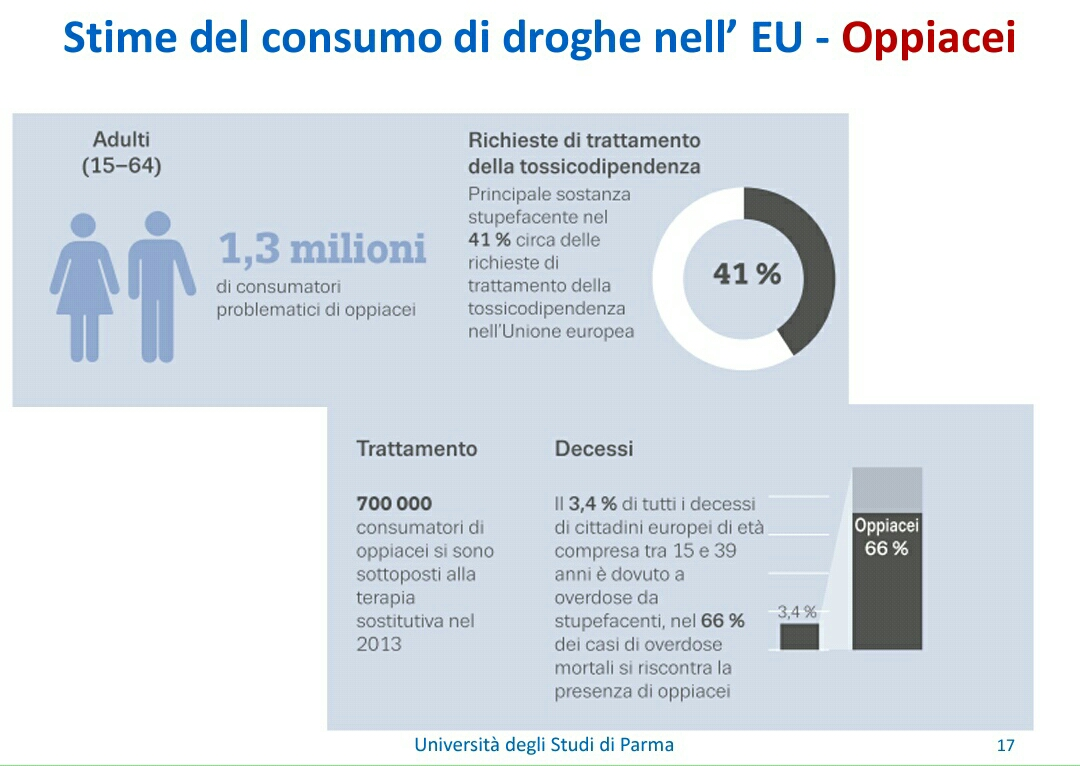
\includegraphics[width=0.7\textwidth]{18/image5.jpeg}
\end{figure}

Per quanto riguarda
l'\textbf{ecstasy}, si rileva un 3,6\% di popolazione utilizzatrice
nell'arco della vita e uno 0,6\% nel corso dell'ultimo anno, che sale
all'1,4\% tra i più giovani.

\begin{figure}[!ht]
\centering
	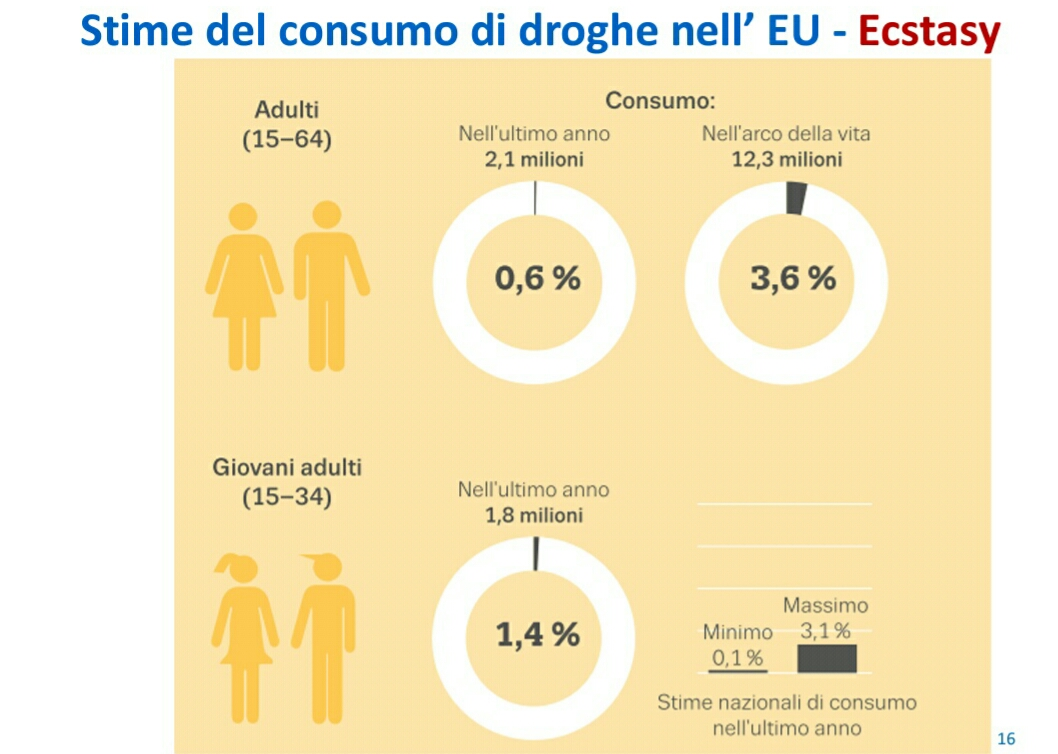
\includegraphics[width=0.7\textwidth]{18/image6.jpeg}
\end{figure}

Da questi dati si evince che il consumo maggiore è all'interno della
popolazione giovane adulta, soprattutto nell'ambito del consumo che
nasce come occasionale.

Vengono forniti anche grafici sui consumi nazionali. Ad esempio, secondo
questo report, per quanto riguarda l'ecstasy, ci sono paesi con un
consumo di 0,1\% fino a paesi con un picco di 3,1\%; inoltre ci dicono
che il 41\% della richiesta di trattamento della dipendenza è da
oppiacei.

Gli Stati Uniti e il Nord Europa prediligono tendenzialmente le droghe
di sintesi, mentre il Sud Europa predilige i cannabinoidi. Tuttavia va
tenuto in considerazione che negli Stati Uniti i dati, stilati dal CDC,
sono raccolti a livello federale, di singolo stato e quindi risultano
più influenzabili e meno affidabili di quelli europei.

In Italia, per le legge, i dati statistici ed epidemiologici sullo stato
delle tossicodipendenze sono oggetto di un rapporto che viene presentato
in Parlamento ogni 12 mesi in riferimento all'anno precedente, al fine
di fornire ai decisori gli strumenti e dei dati sui quali basare le
politiche, ricordando che questo fenomeno ha delle ripercussioni non
indifferenti sul sistema sanitario. Inoltre i dati di letteratura
sull'efficacia della prevenzione dimostrano come tutti gli interventi
che cercano di curare questo fenomeno siano per gran parte inefficaci.
La relazione parlamentare parla di ``misure antidroga'', che possono
colpire:
\\\\
\begin{enumerate}
\def\labelenumi{\arabic{enumi}.}
\item
  L'offerta, ovvero chi mette disposizione la droga;
\item
  La domanda, ossia il consumo.
\end{enumerate}

Per bloccare l'offerta si può agire sui sistemi di controllo (guardia di
finanza), sulle ripercussioni penali e sull'inasprimento delle pene. Per
ridurre la domanda, invece, si può puntare sull'educazione sanitaria e
sulla promozione della salute, ad esempio con video e brochure,
attraverso la prevenzione primaria. Se, invece, si cerca di agire su chi
già fa uso di sostanze si parla di prevenzione secondaria.

\begin{figure}[!ht]
\centering
	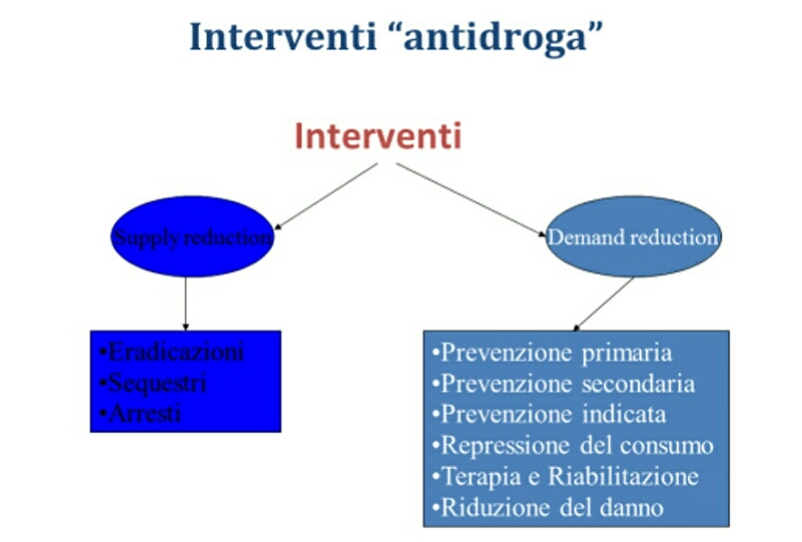
\includegraphics[width=0.7\textwidth]{18/image7.jpeg}
\end{figure}

Arrivare ad agire su quelli che sono i determinanti più prossimali
dell'individuo potrebbe non essere efficace. Tenete presente che i
determinanti di salute sono molti e se agissimo anche su quelli più
distali, come il contesto socio-economico potremmo avere ripercussioni
specifiche sul problema sanitario su cui si vuole agire. L'efficacia
degli interventi soprattutto sui determinanti prossimali attualmente è
molto bassa.
\\\\
Qual è la risposta sociale-sanitaria ai problemi legati alla droga?

\begin{figure}[!ht]
\centering
	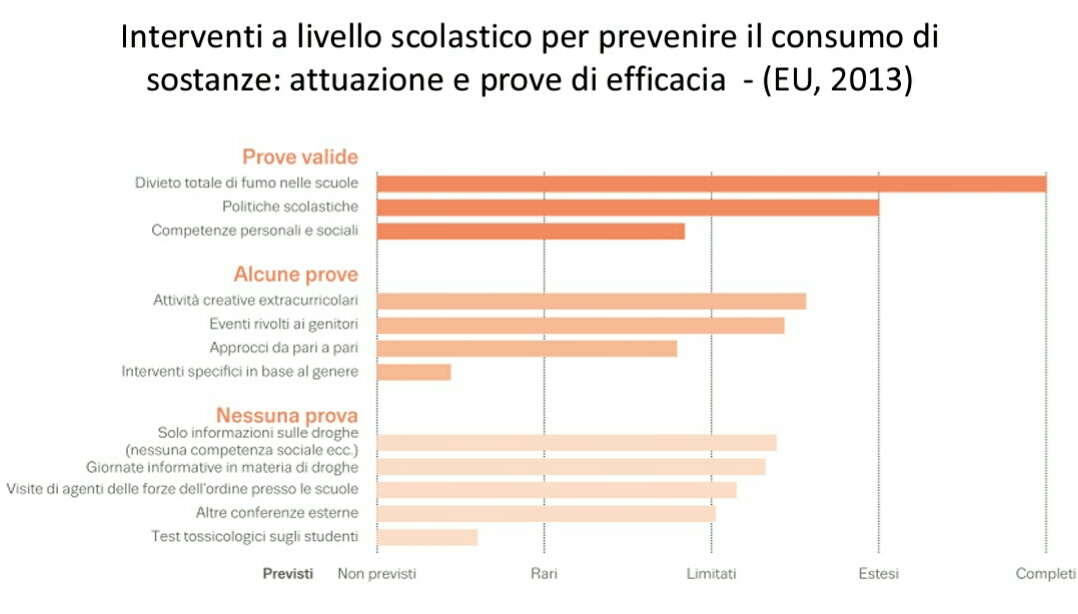
\includegraphics[width=0.7\textwidth]{18/image8.jpeg}
\end{figure}

Esistono dati sull'efficacia
specifica di varie misure di controllo a livello scolastico, come ad
esempio il divieto totale di fumo nelle scuole, le politiche scolastiche
generali, le attività ricreative extra-curricolari, gli eventi per i
genitori, gli approcci da pari a pari, la distribuzione di materiale
informativo, le giornate informative in materia di droga, le visite
delle forze dell'ordine, i test tossicologici agli studenti\ldots{}

Questo è un tema sociale molto sentito dalla popolazione ma c'è una
mancanza di coerenza e coesione tra quelli che sono gli interventi di
provata efficacia e i dati dell'efficacia di questi interventi, che
indicano in realtà degli scarsi risultati.

In occasione della giornata mondiale della prevenzione e del controllo
dell'utilizzo di droghe l'agenzia delle Nazioni Unite per le droghe ha
lanciato l'iniziativa UNODC YOU, che prevede l'assegnazione di fondi ad
associazioni no profit, che lavorano con giovani a basso e medio reddito
con l'obiettivo di incoraggiare i giovani ad assumere un ruolo più
attivo nella loro comunità, attraverso la creazione di ambienti che
siano meno inclini a portare i soggetti giovani al consumo di sostanze.

Sempre per quanto riguarda le politiche a livello globale, c'è stata
quest'anno una sessione speciale dell'assemblea delle Nazioni Unite, che
si è espressa sul problema del consumo di droghe e su tutti i problemi
politici, economici e sanitari correlati a livello globale.

\subsection{La dipendenza da gioco d'azzardo}


All'interno delle dipendenze rientra anche quella che viene codificata
dall'ultima versione del DSM come LUDOPATIA, che è un fenomeno tangibile
e in aumento. Ci sono articoli di giornale anche recentissimi che
sottolineano quanto sia in aumento questa pratica e quanto sia
trasversale sul territorio. A livello italiano i determinanti di questo
fenomeno possono essere l'aumento della disoccupazione, le insicurezze
sociali e le condizioni di disagio socio-economico, soprattutto negli
strati medio-bassi della popolazione.

Per ludopatia o GAP (gioco d'azzardo patologico) si intende l'incapacità
di resistere all'impulso di giocare d'azzardo o fare soldi, nonostante
l'individuo che ne è affetto sia consapevole che questo può portare a
gravi conseguenze. Non è solo un fenomeno sociale, ma è una vera e
propria patologia, che rende incapaci di resistere all'impulso di
giocare d'azzardo o fare scommesse. Inoltre, nonostante la ludopatia
provochi una dipendenza che è solo psicologica, viene codificata dal DSM
come comportamento problematico persistente o ricorrente, legato al
gioco d'azzardo che porta disagio e compromissione clinicamente
significativi come indicato dall'individuo che presenta 4 o più delle
seguenti condizioni entro un periodo di 12 mesi:

\begin{enumerate}
\def\labelenumi{\arabic{enumi}.}
\item
  Ha bisogno di quantità crescenti di denaro per giocare al fine di
  ottenere l'eccitazione desiderata;
\item
  È irrequieto, irritabile se tenta di smettere di giocare;
\item
  Ha fatto ripetuti sforzi infruttuosi per controllare/ridurre/smettere
  di giocare
\item
  È ossessionato dal gioco d'azzardo (pensieri persistenti)
\item
  Spesso gioca d'azzardo anche quando si sente a disagio (indifeso,
  colpevole, ansioso, depresso)
\item
  Dopo aver perduto denaro al gioco d'azzardo spesso torna un'altra
  volta per tentare di rimediare alle proprie perdite
\item
  Mente per occultare l'entità del coinvolgimento
\item
  Ha messo in pericolo o perduto una relazione significativa, il lavoro
  o l'opportunità di studio/carriera a causa del gioco
\item
  Conta su gli altri per procurare il denaro necessario
\end{enumerate}

Con quattro di questi elementi si fa diagnosi con una gravità che può
essere lieve (4-5 criteri), moderata (6-7), grave (8-9).
\subparagraph{Qual'è la distribuzione?}


Globalmente i dati dicono che secondo stime americane il 2-4\% della
popolazione è affetto da ludopatia. In particolare negli uomini il
disturbo sembra iniziare in adolescenza, mentre nelle donne l'insorgenza
è più tardiva.

Le componenti di questa patologia sono in parte familiari o genetiche
(in via di ricerca) e in parte legate ai determinanti, ovvero ai fattori
ambientali, che possono favorire una determinata inclinazione.

L'ultimo rapporto dell'Emilia Romagna dice che a livello regionale il
gioco d'azzardo comporta una spesa media procapite di oltre 1800 euro
all'anno tra i soli individui maggiorenni. Se rapportiamo la spesa per
il gioco al PIL al primo posto si trova Rimini, poi Reggio Emilia,
Modena, Parma e Ferrara. Solo alcune province si attestano sotto al 4\%
del PIL. Si tratta di indicatori significativi per valutare
l'indebitamento legato a comportamento patologico e il rischio di usura,
che deriva da questa propensione al gioco.

\begin{figure}[!ht]
\centering
	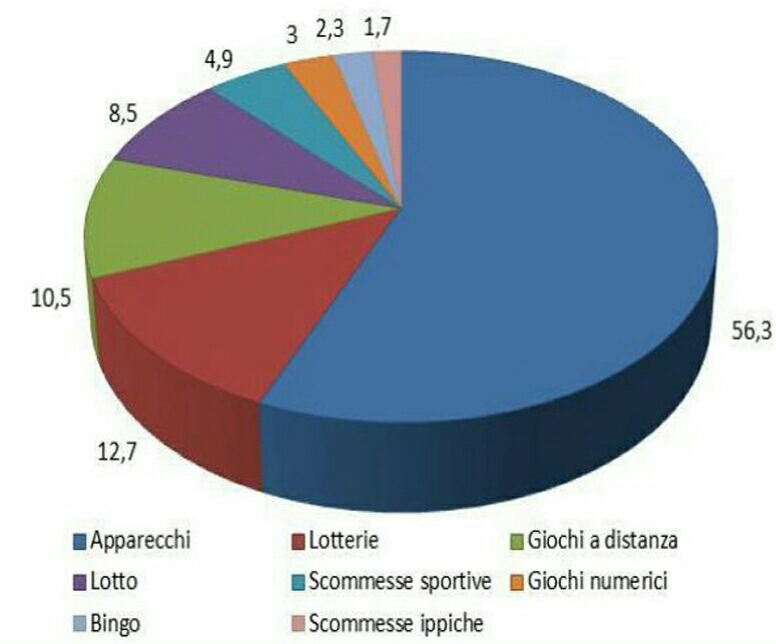
\includegraphics[width=0.7\textwidth]{18/image9.jpeg}
\end{figure}

Infatti gli effetti della ludopatia
sono svariati: problemi finanziari, compromissione delle relazioni
personali, perdita del lavoro e sviluppo di dipendenze (droga,
alcol...). Quest'ultimo punto è legato al fatto che di solito le
patologie associate a dipendenza mentale tendono a presentarsi insieme,
come comorbilità. Di recente la normativa ha inserito la ludopatia nei
livelli essenziali di assistenza con riferimento alle prestazioni di
prevenzione, cura e riabilitazione, rivolte alle persone affette da
questa patologia.

Questi sono dei dati dell'Eurobet, che è un sondaggio europeo che dice
quali sono i dispositivi più utilizzati da chi ha un approccio
dipendente:

\begin{itemize}
\item
  Slot machine: oltre 60\%
\item
  Lotterie (inclusi gratta e vinci ecc\ldots{}): 13\%
\item
  Giochi a distanza: 10\% (in particolare, il gioco online, soprattutto
  per il fatto che garantisce l'anonimato, sta acquisendo molti punti)
\end{itemize}

A seguire in ordine:

\begin{itemize}
\item
  Lotto
\item
  Scommesse sportive
\item
  Giochi numerici (es. bingo)
\end{itemize}

I giocatori d'azzardo vengono classificati in giocatori sociali, ovvero
quelli che giocano ai casinò saltuariamente, problematici e patologici,
che sono quelli che rispondo ai criteri del DSM.

Il piano nazionale di prevenzione prevede 10 macro-obiettivi, tra cui
uno riguarda le dipendenze, sia a livello di sostanze che di
comportamenti, identificando come fattori di rischio in Italia la
percezione del rischio, lo stile di vita e la mancanza di competenze di
individui ed operatori. Il piano identifica alcune strategie, tra cui
alcune integrate ed interistituzionali (sistema scolastico e sanitario)
per valorizzare e promuovere le capacità personali dei giovani in
termini di autostima, resistenza e resilienza, altre intersettoriali per
prevenire e ridurre il disagio sociale e familiare.

Alcuni esempi di prevenzione, proposti da piano nazionale, sono:
\begin{itemize}


\item 
-proposte di legge
\item 
-riduzione dell'offerta, sia in termine di volumi che di punti vendita
\item 
-definizione un sistema di regole sull'apertura di sale giochi
\item 
-educazione sanitaria e comunicazione
\item 
-procedimenti di tipo normativo
\end{itemize}

\begin{figure}[!ht]
\centering
	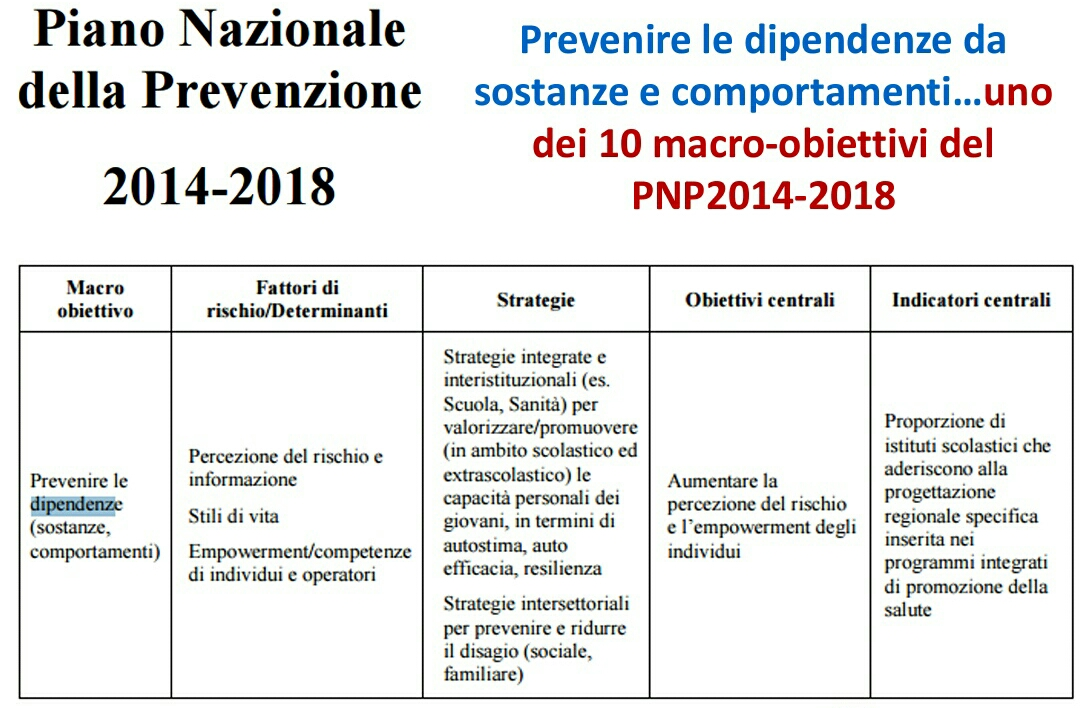
\includegraphics[width=0.7\textwidth]{18/image10.jpeg}
\end{figure}


Infine, esistono altre nuove forme di dipendenza: energy drink, shopping
compulsivo\ldots{}

\section{Comportamenti sessuali a rischio}


Tra i determinanti ci sono anche i comportamenti sessuali, che sono
fattori di rischio per le infezioni sessualmente trasmesse, ma anche per
alcune neoplasie, quali l'epatocarcinoma e il carcinoma della cervice
uterina e dell'orofaringe da HPV. Questi sono tra i pochissimi tumori
prevenibili con opere di prevenzione primaria, come la vaccinazione
(tipico argomento d'esame richiesto all'orale). Inoltre i comportamenti
sessuali a rischio hanno come indicatore anche le gravidanze
indesiderate.

Nel Regno Unito soldi vengono utilizzati a scopo di ricerca per fare
delle indagini sulle abitudini sessuali di tutta la popolazione perché
questo fornisce delle informazioni utili agli interventi di prevenzione.
Al contrario, in Italia non ci sono fondi né tantomeno iniziative per
fare uno studio simile sulle abitudine sessuali degli italiani. Sarebbe
interessante analizzarle anche in relazione a quelle degli altri stati
europei perché c'è una componente culturale e di educazione sessuale,
che potrebbe giustificare grosse differenze tra stato e stato.

\begin{figure}[!ht]
\centering
	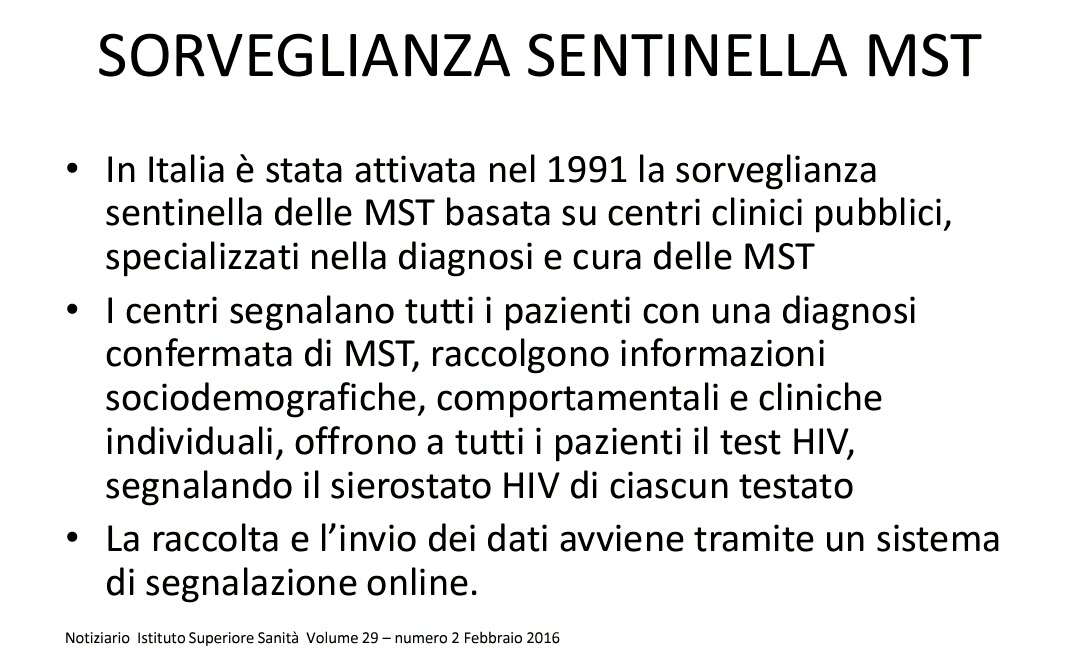
\includegraphics[width=0.7\textwidth]{18/image11.jpeg}
\end{figure}

Lo studio inglese, pubblicato sul
Lancet, analizza per coorte di nascita il numero medio di partner
sessuali di sesso opposto nella vita nella popolazione adulta tra i 16 e
i 44 anni. Tra le femmine, si passa da 3,7 nel 1990 ad un valore quasi
duplicato nell'ultima rilevazione. Tra i maschi, nonostante ci sia un
bias d'informazione, si rileva lo stesso trend di aumento.

Il sistema di sorveglianza in Italia rileva un trend di aumento delle
infezioni sessualmente trasmissibili.

\begin{figure}[!ht]
\centering
	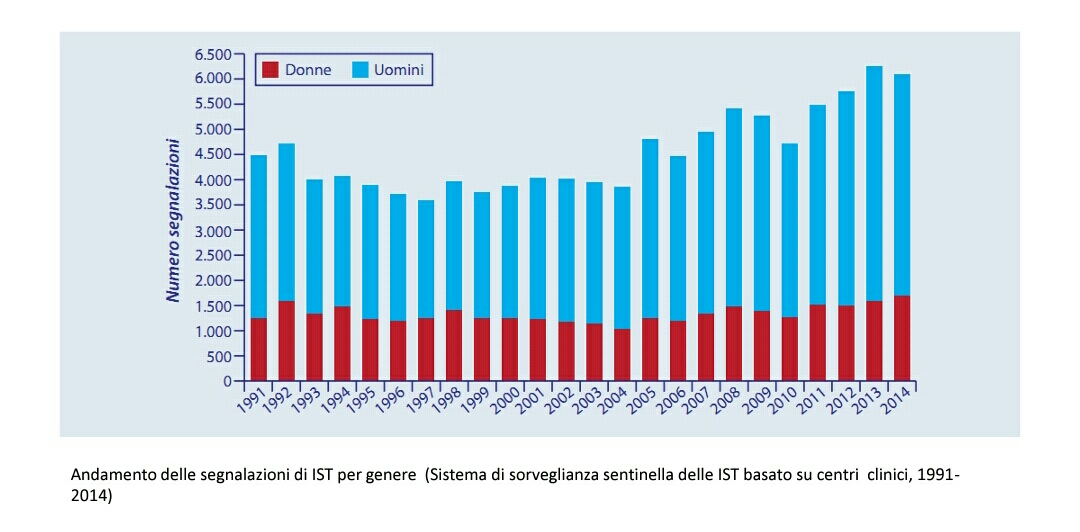
\includegraphics[width=0.7\textwidth]{18/image12.jpeg}
\end{figure}

\begin{figure}[!ht]
\centering
	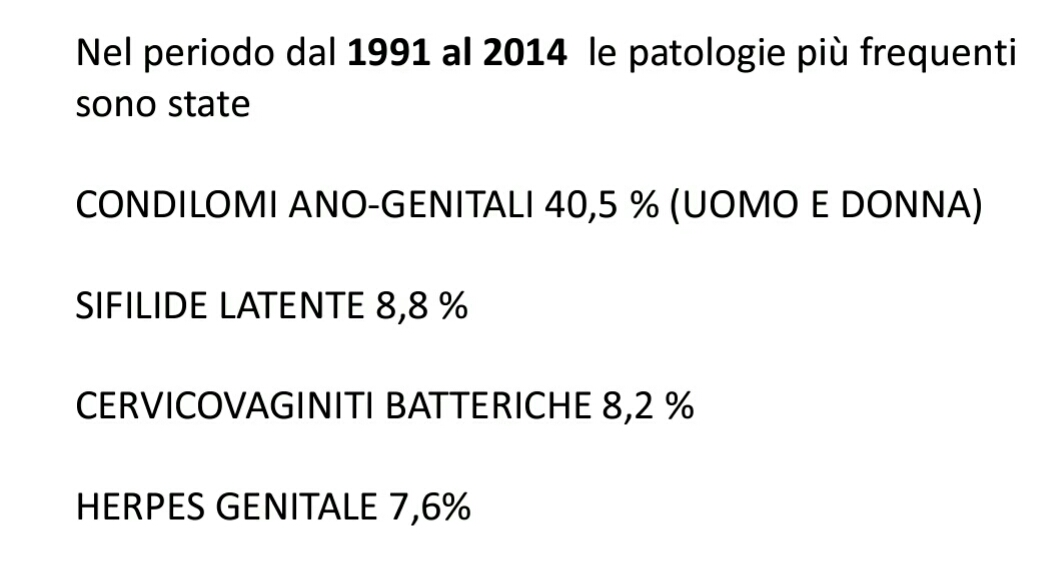
\includegraphics[width=0.7\textwidth]{18/image13.jpeg}
\end{figure}

